\documentclass[a4paper,11pt]{article}
\usepackage{pos}

\usepackage{caption}
\usepackage{float}
\usepackage[lofdepth=1,lotdepth]{subfig}

\usepackage[noabbrev, capitalise, nameinlink]{cleveref}  % reference object types automatically

% until reviewed
\usepackage{lineno}
\linenumbers

\title{Search for heavy neutral lepton production and decay with the IceCube Neutrino Observatory}
%% \ShortTitle{Short Title for header}

\manuallySeparateAuthors
\author*[a]{Leander Fischer}
\author[b]{and Julia Book}
\author{for the IceCube collaboration}


\affiliation[a]{DESY, D-15738 Zeuthen, Germany}
\affiliation[b]{Harvard University, Cambridge, MA 02138, USA}

\emailAdd{leander.fischer@desy.de}
\emailAdd{jbook@g.harvard.edu}

\abstract{
Sterile neutrinos are a well motivated objective of Beyond Standard Model (BSM) searches. Extensions to the Standard Model (SM) including right handed (sterile) neutrinos pose a viable explanations for the origin of neutrino masses and they could solve a variety of additional open questions in physics such as neutrino oscillation anomalies, the nature of dark matter, and baryon asymmetry. Multiple models posit the existence of a GeV-scale, sterile neutrino (also called a Heavy Neutral Lepton - HNL), which can interact with the SM particles through different mechanisms. The HNL can therefore be produced from and decay into known particles. If the production, from atmospheric neutrino up-scattering, and the HNL's subsequent decay happen inside the IceCube detector, it can produce a unique double-cascade signature, which can be utilized to search for GeV-scale HNLs at atmospheric neutrino energies. Focusing on the flux of atmospheric muon neutrinos that oscillate into tau neutrions, the less constrained $\tau$-sterile space can be explored. We present the analysis approach of studying HNLs in the mass range of 0.1-3 GeV, by searching for low-energy double-cascade topologies with the IceCube DeepCore detector.
}

\FullConference{%
  41st International Conference on High Energy physics - ICHEP2022\\
  6-13 July, 2022\\
  Bologna, Italy
}

\begin{document}
\maketitle


\section{Introduction}


Extensions to the Standard Model (SM) adding heavy neutral leptons (HNLs) provide a good explanation to the origin of neutrinos masses through type-I seesaw mechanisms \cite{10.1143/PTP.64.1103}. While the mixing with $\nu_{e,\mu}$ is strongly constrained ($|U_{\alpha4}^2| \lesssim 10^{-5}-10^{-8}, \alpha=e,\mu$), the mixing with $\nu_{\tau}$ is much harder to probe, due to the difficulty of producing and detecting tau neutrinos. \cref{fig:hnl_limits_and_decay_widths} shows the current limits on the $\tau$-sterile for HNL masses between $0.1-10\,$GeV. As was first pointed out in \cite{Coloma:2017ppo}, the atmospheric neutrino flux observed in IceCube offers offer a way to constrain the neutrino-HNL mixing parameters. Using the large fraction of atmospheric $\nu_{\mu}$ events that oscillate into $\nu_{\tau}$ until they reach the detector \cite{IceCube:2019dqi}, the less constrained $\tau$-sterile space can be explored.



\begin{figure}[h]
  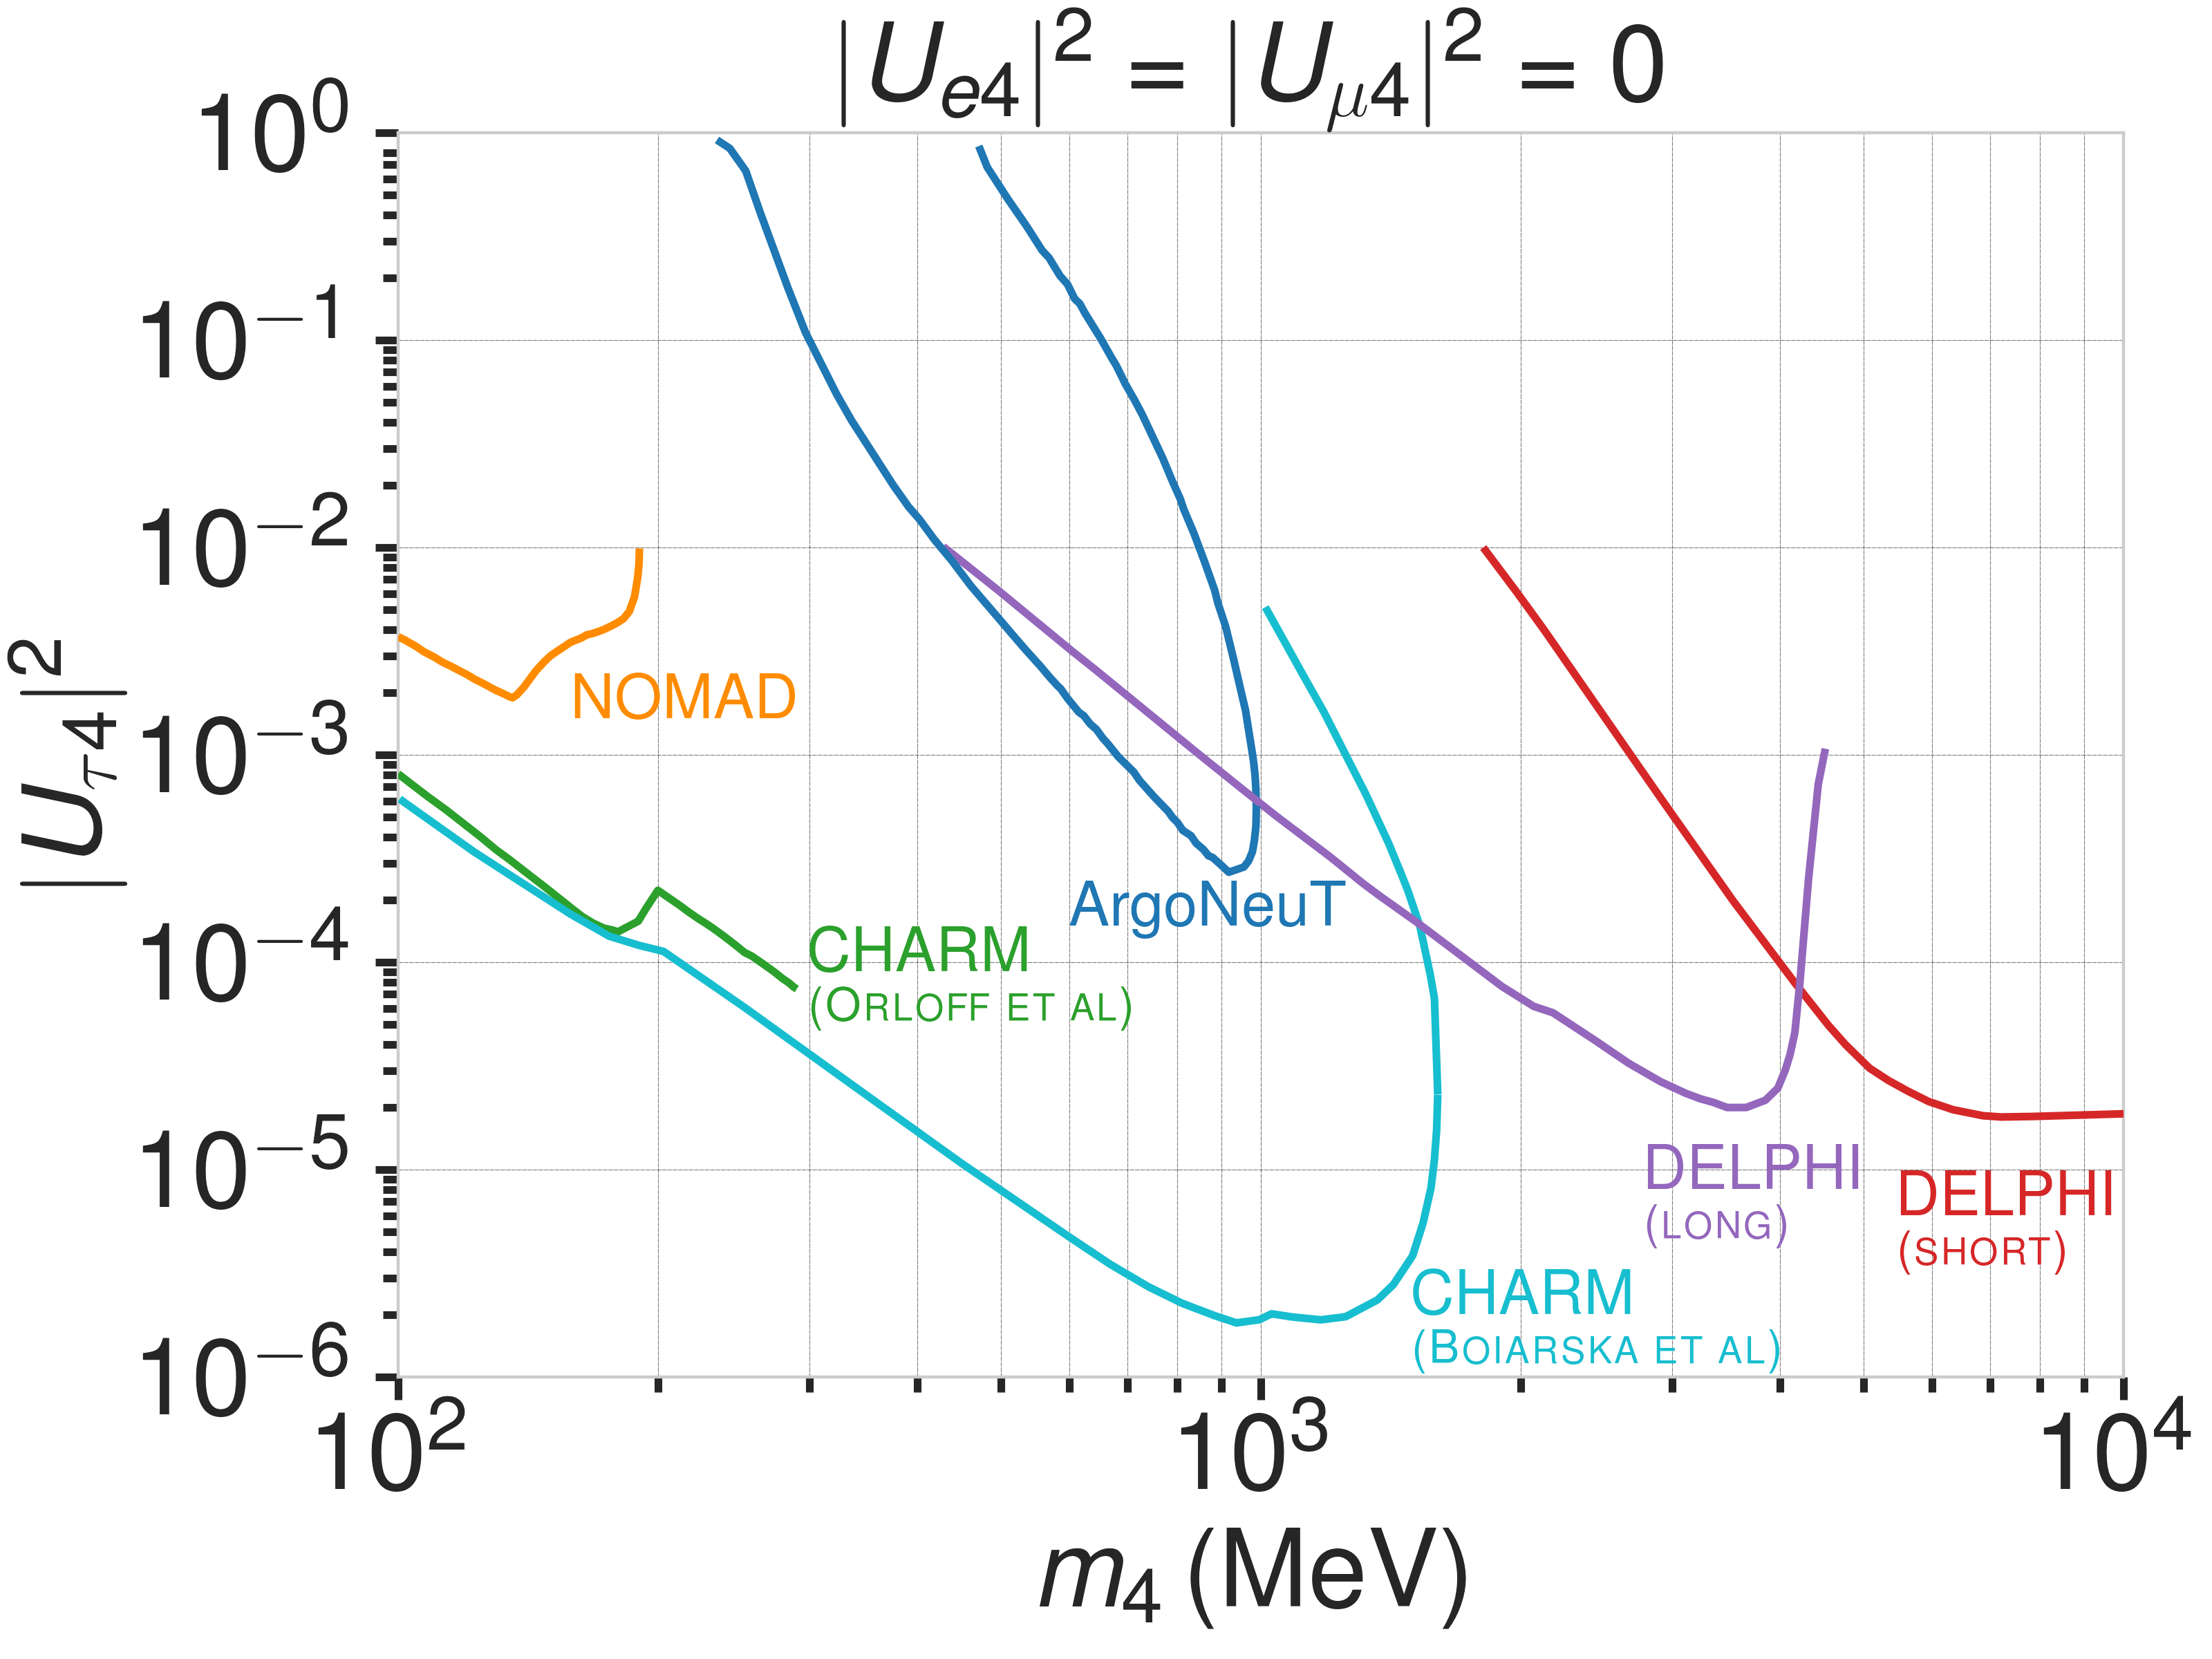
\includegraphics[width=.50\linewidth]{figures/UtauN_custom_plots_LF_grid_white.png}
  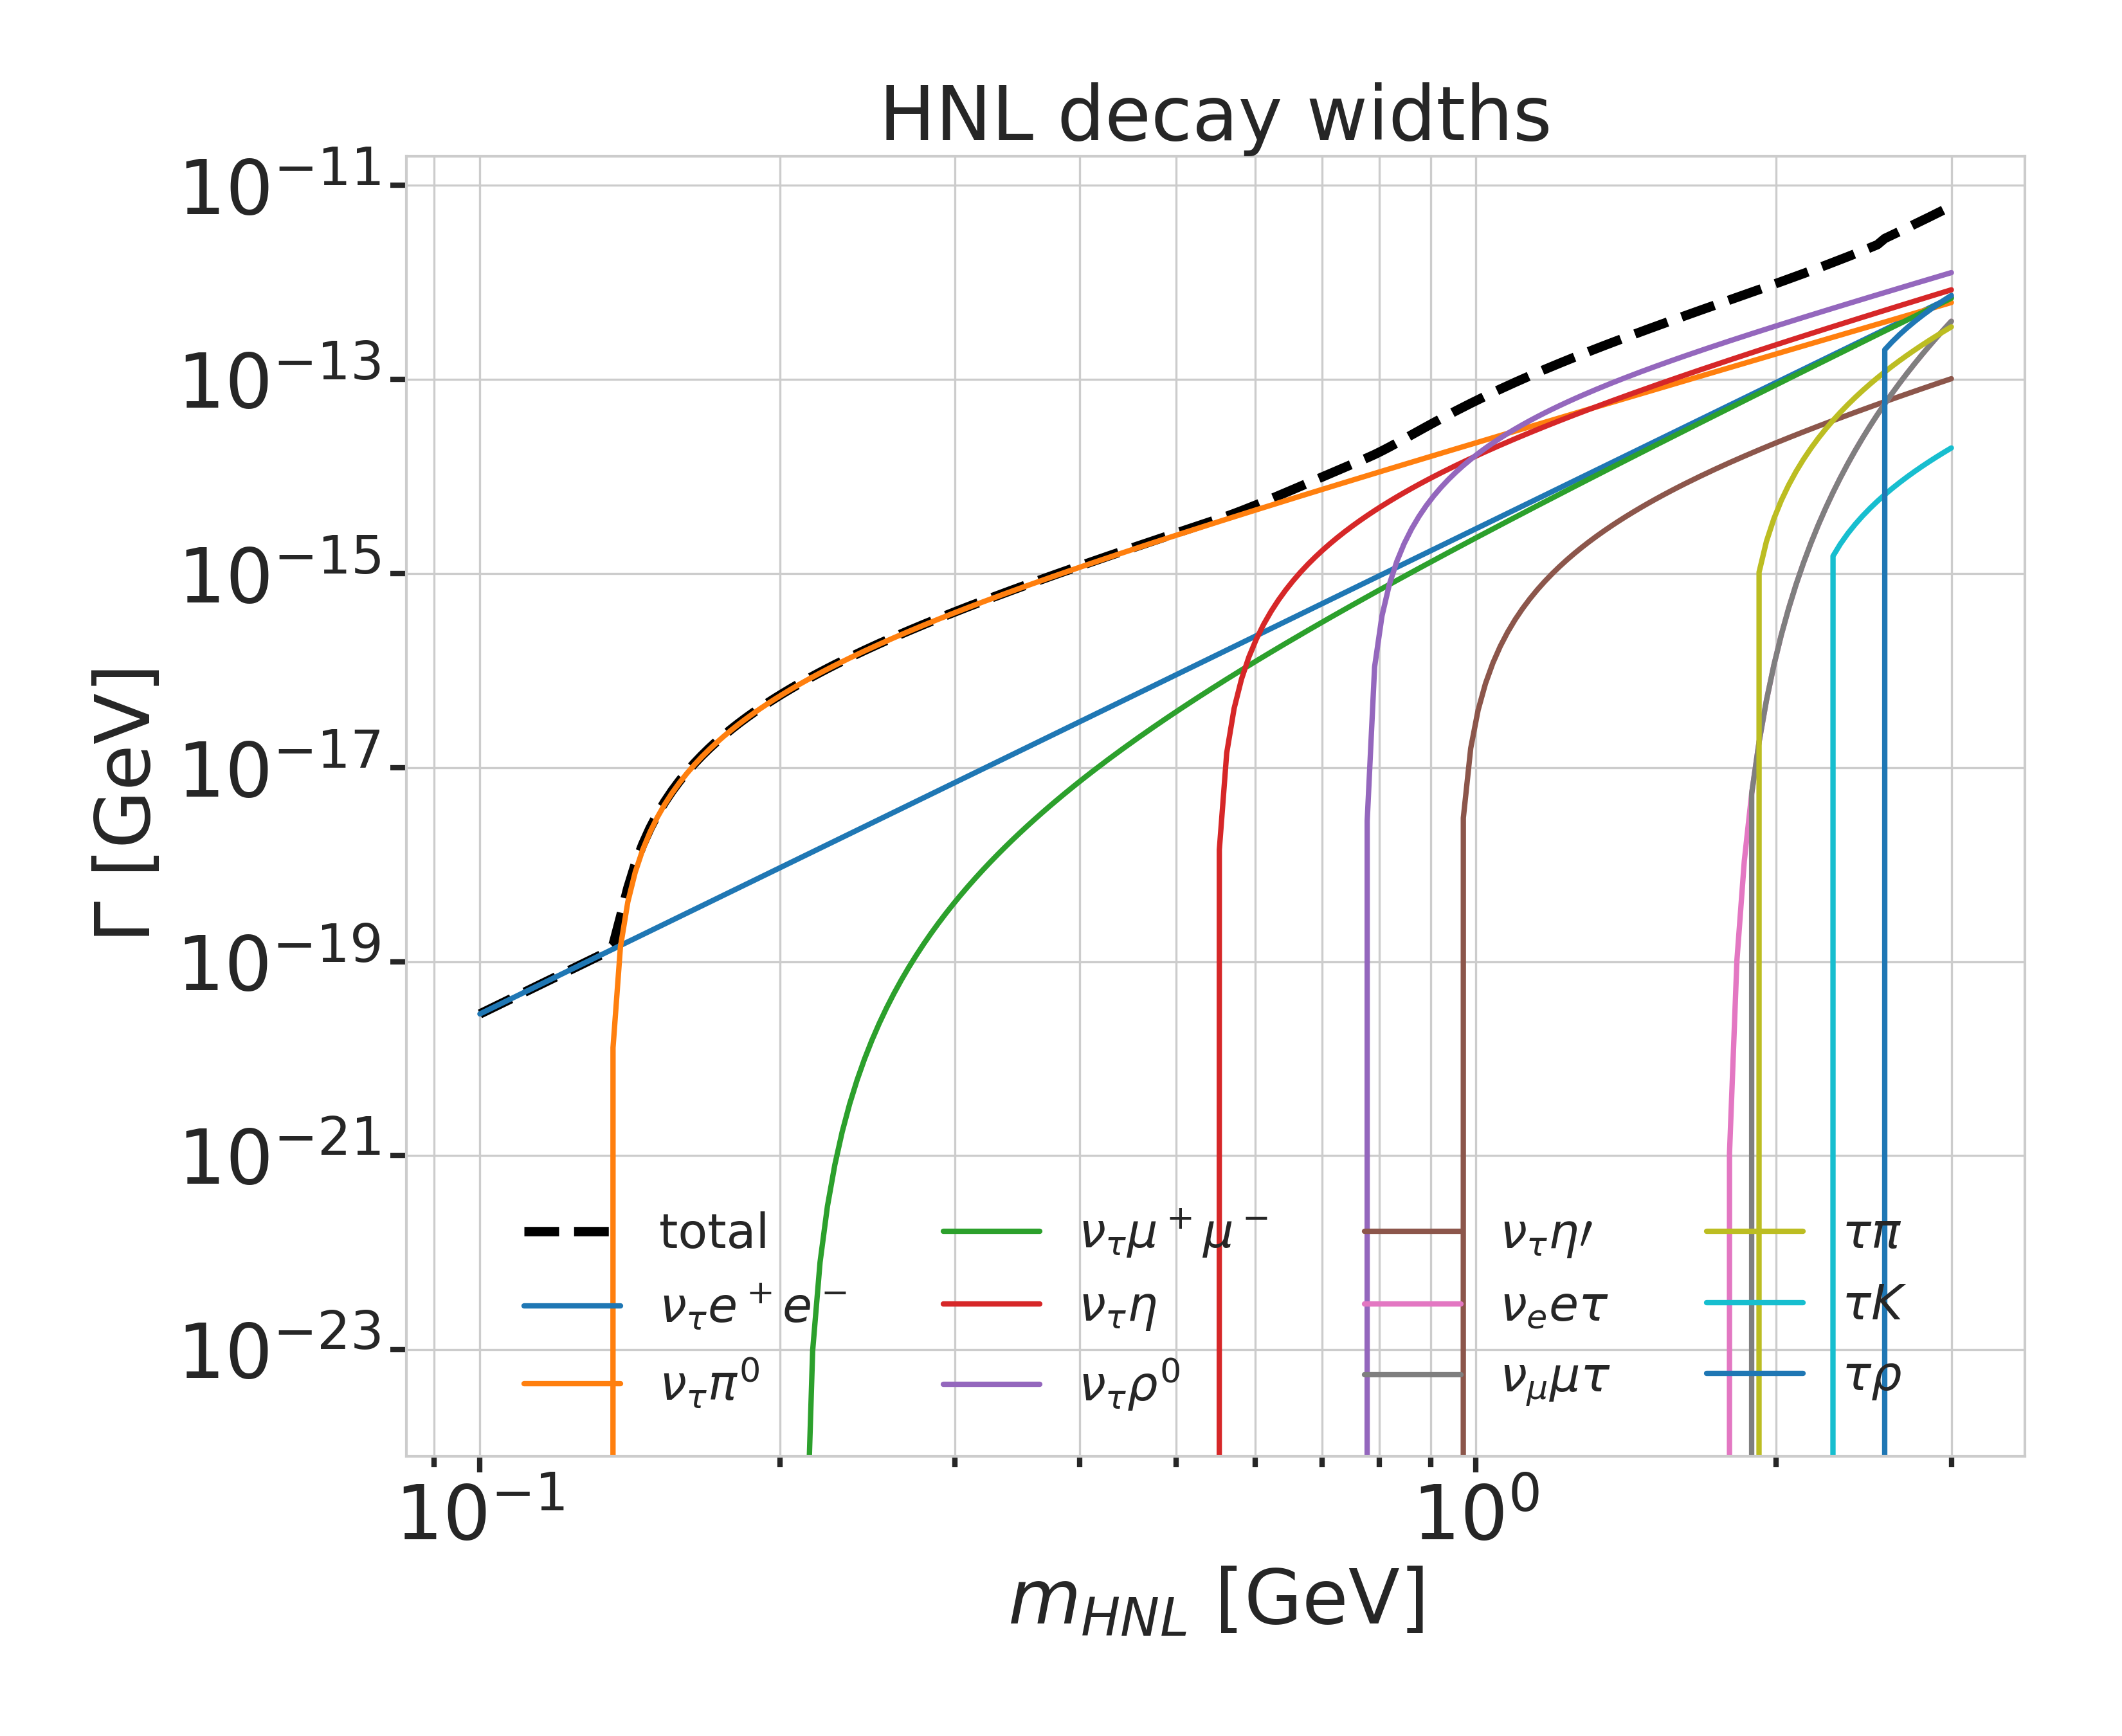
\includegraphics[width=.47\linewidth]{figures/hnl_decay_widths_log.png}
  \label{fig:hnl_visible_decay_widths}
  \caption{Current $|U_{\tau4}^2|$ limits (left) from NOMAD \cite{NOMAD:2001eyx}, ArgoNeut \cite{ArgoNeuT:2021clc}, CHARM \cite{Orloff:2002de, Boiarska:2021yho}, and DELPHI \cite{DELPHI:1996qcc} and decay widths of visible decay modes in IceCube (right) calculated based on the results from \cite{Gorbunov:2007ak}.}
  \label{fig:hnl_limits_and_decay_widths}
\end{figure}


\section{IceCube DeepCore}

The IceCube Neutrino Observatory \cite{Aartsen:2016nxy} is located at the geographic South Pole and consists of 5160 Digital Optical Modules (DOMs), deployed into the antarctic glacial ice at depths between 1.45\,km and 2.45\,km. It is an ice Cherenkov telescope instrumenting a volume of about 1\,km$^{3}$. The ice is used as interaction and detection medium, simultaneously, where interacting neutrinos can produce charged secondary particles, which themselves can emit Cherenkov photons detectable by the DOMs. The DOMs are arranged on a nearly-hexagonal array, as shown in \cref{fig:icecube_array}, with 125\,m horizontal and 17\,m vertical spacing in IceCube and a closer 42-72\,m horizontal of 7\,m vertical spacing in the denser, bottom-center part of the array, called DeepCore \cite{IceCube:2011ucd}. While IceCube targets the detection of astrophysical neutrinos with energies above $\sim$100\,GeV, DeepCore can measure neutrino interactions down to a few GeV, due to its closer spacing in regions with very good optical properties of the ice. This allows the measurement of atmospheric neutrino oscillations that occur mainly occur in the 10-50\,GeV region. The location of DeepCore is also indicated in \cref{fig:icecube_array}, which also shows the absorption properties of the ice with respect to depth.

\begin{figure}[h]
  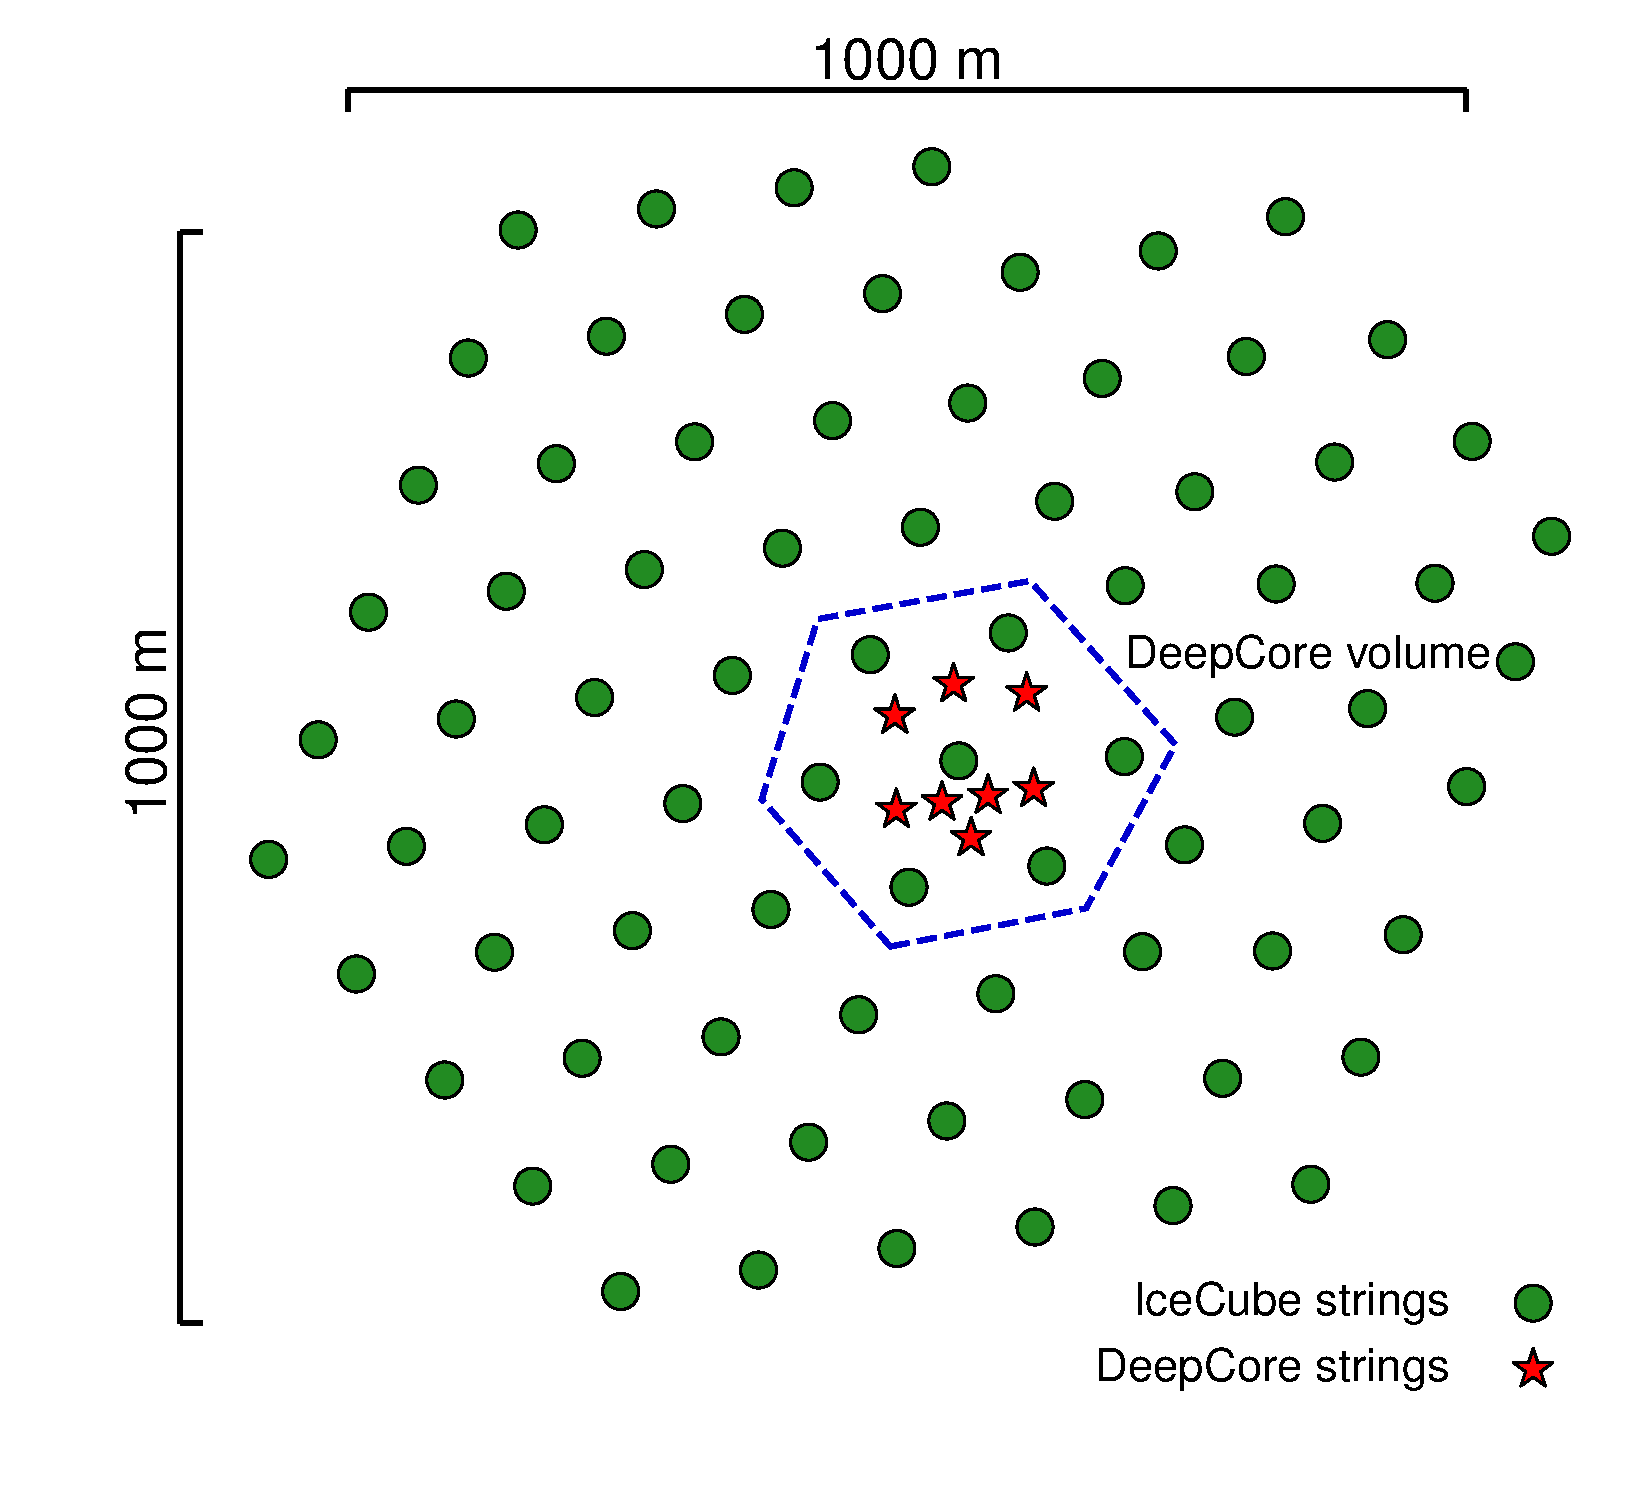
\includegraphics[width=.43\linewidth]{figures/icecube_top_view_bw.pdf}
  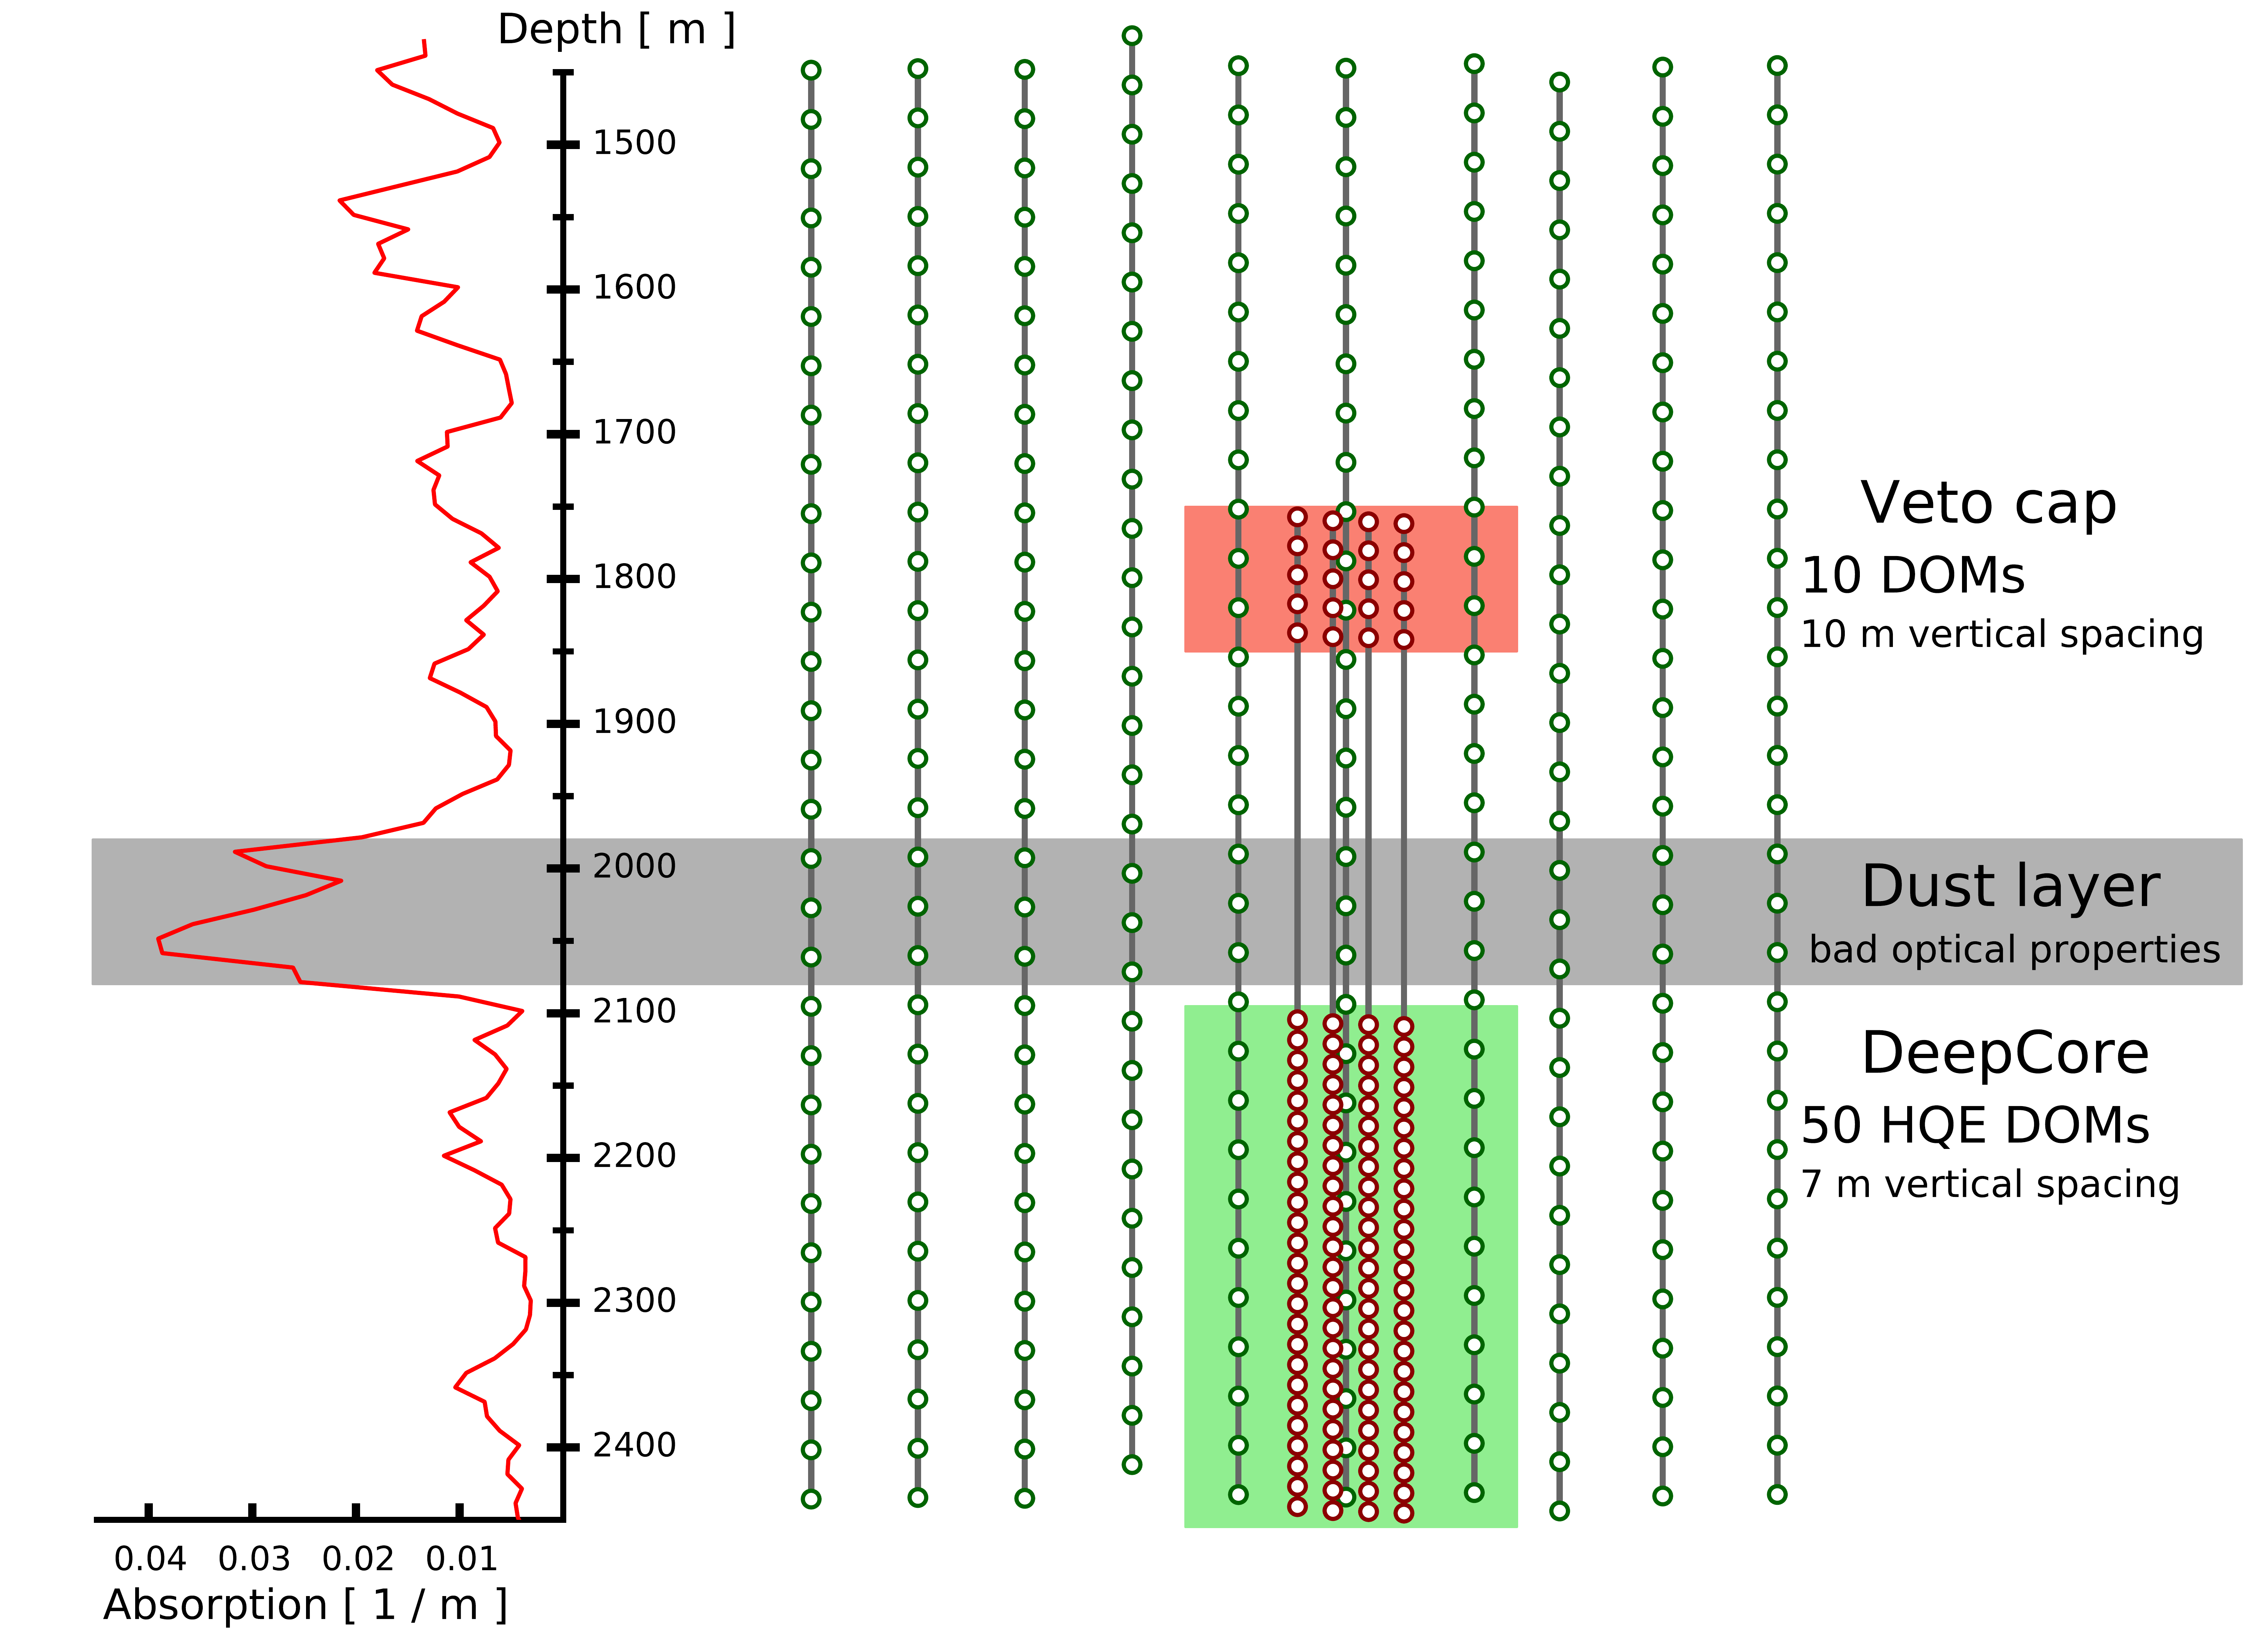
\includegraphics[width=.52\linewidth]{figures/DeepCore_sideview.png}
  \caption{Top-view (left) and side-view (right) of the IceCube and DeepCore array. The side-view also shows the ice absorption at different depths.}
  \label{fig:icecube_array}
\end{figure}

The two observable low energy event topologies in IceCube DeepCore are \textit{tracks} and \textit{cascades}. Tracks are elongated light emission patterns, produced by long-lived muons, mainly originating from $\nu_{\mu}$ CC interactions or cosmic ray air showers, with a subdominant component from $\nu_{\tau}$ CC interactions (BR of $\tau\rightarrow\mu$ $\sim 17\%$ \cite{PhysRevD.98.030001}). Cascades are roughly point-like, spherical light emissions, produced by electromagnetic and hadronic showers. They are produced by $\nu_{e}$ and most $\nu_{\tau}$ CC interactions, as well as NC interactions of all flavours.

% \begin{figure}[h]
%   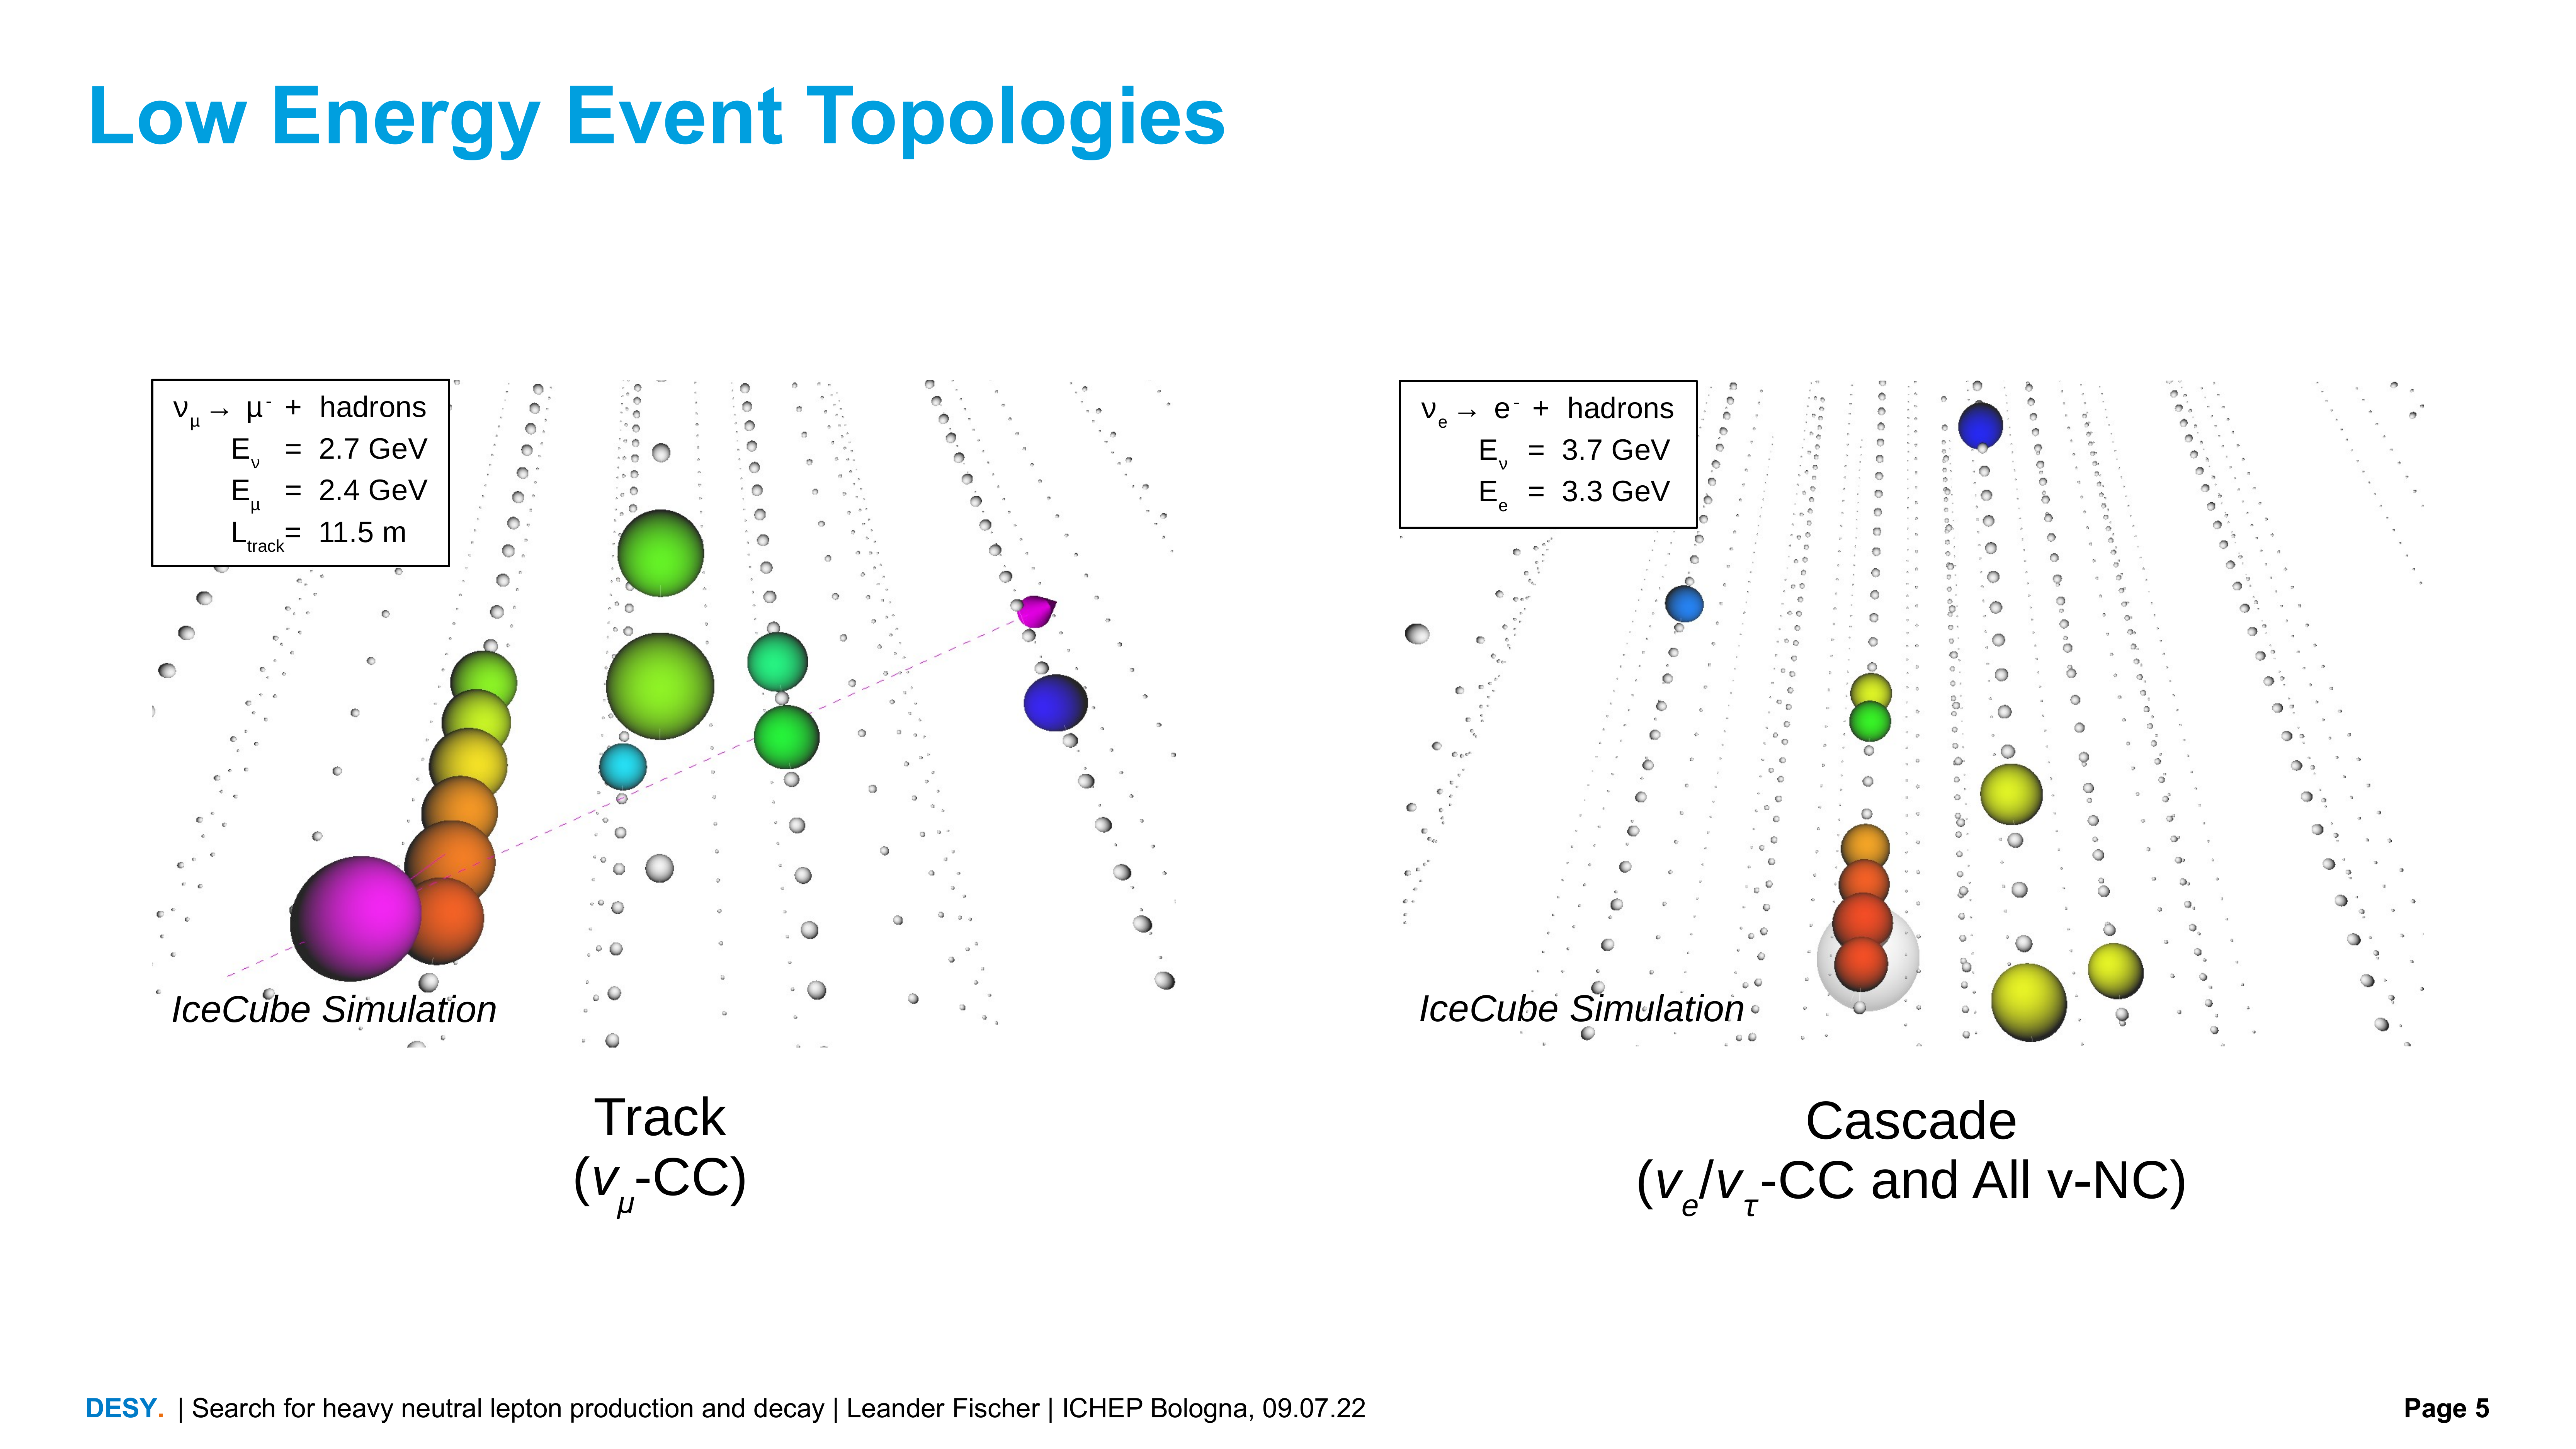
\includegraphics[trim = 2cm 3cm 2cm 5cm, clip, width=1.0\linewidth]{figures/event_views.png}
%   \caption{Example of low energy event topologies in IceCube DeepCore. The color of the spheres indicates the arrival time of the photons while its size is relative to the number of photons that were detected.}
%   \label{fig:low_energy_eventviews}
% \end{figure}


\begin{figure}[h]
    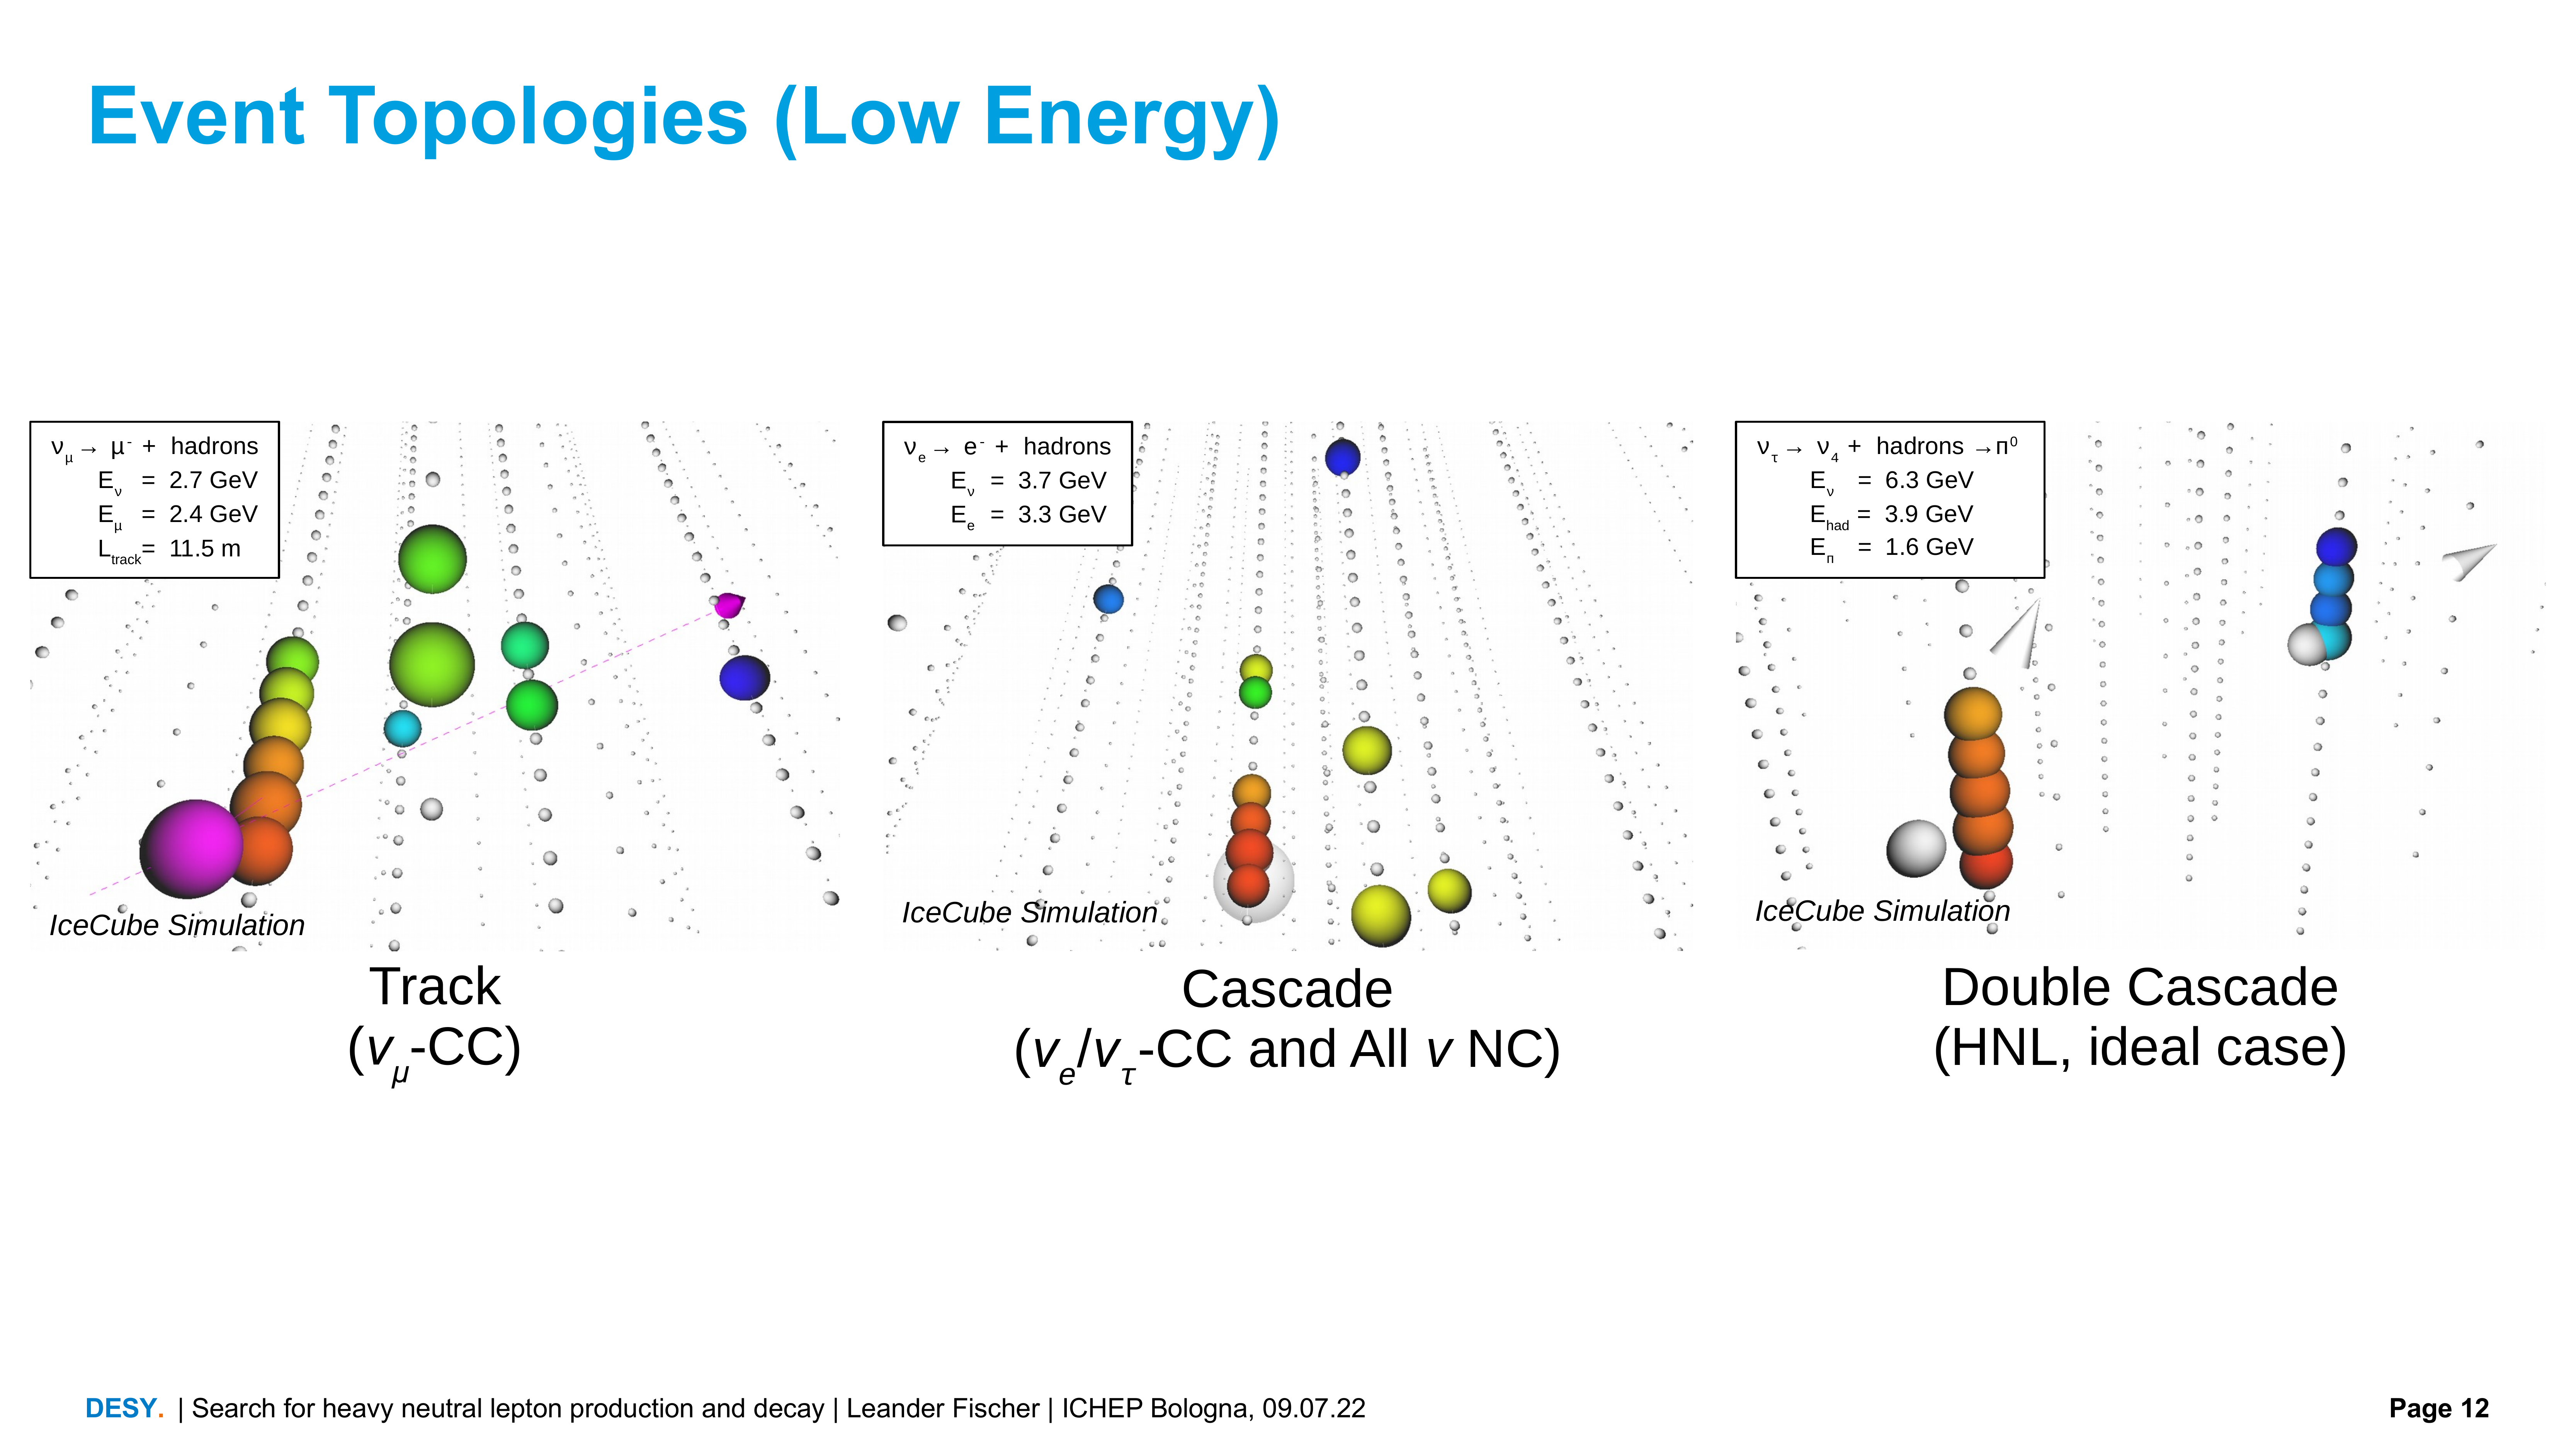
\includegraphics[trim = 0cm 4.5cm 0cm 5.5cm, clip, width=1.0\linewidth]{figures/event_views_all_three.png}
    \caption{Example of low energy event topologies in IceCube DeepCore. The color of the spheres indicates the arrival time of the photons while its size is relative to the number of photons that were detected.}
    \label{fig:low_energy_eventviews}
  \end{figure}


\section{Neutrino Oscillations} \label{sec:neutrino_oscillations}

\begin{itemize}
    \item mass/flavor mixing
    \item testable phase space (ennergy/zenith)
    \item 10 year data sample + rates
    \item IC/DC oscillation results (OVS, hight stats prediction)
\end{itemize}


\section{Heavy neutral lepton search}

\textbf{Snippets:}
\begin{itemize}
    \item existence of a fourth, massive neutrino that would not be charged under any of the SM gauge groups
    \item mixing with SM neutrinos, through extended PMNS matrix
    \item goal of this work it to (first) probe the $|U_{\tau4}^2|$ mixing parameter
    \item select events in DeepCore targeting atmospheric neutrinos and rejecting muons and noise
\end{itemize}




\begin{itemize}
    \item model details
    \item double cascade signatures (up scattering, decay (decay modes))
    \item low energy event signature (double cascade)
    \item nutau detection channel (mass-energy-mixing-decay length relation)
    \item issues/takeaways
    \item envisioned analysis principle
\end{itemize}


% \begin{figure}
%   \centering
%   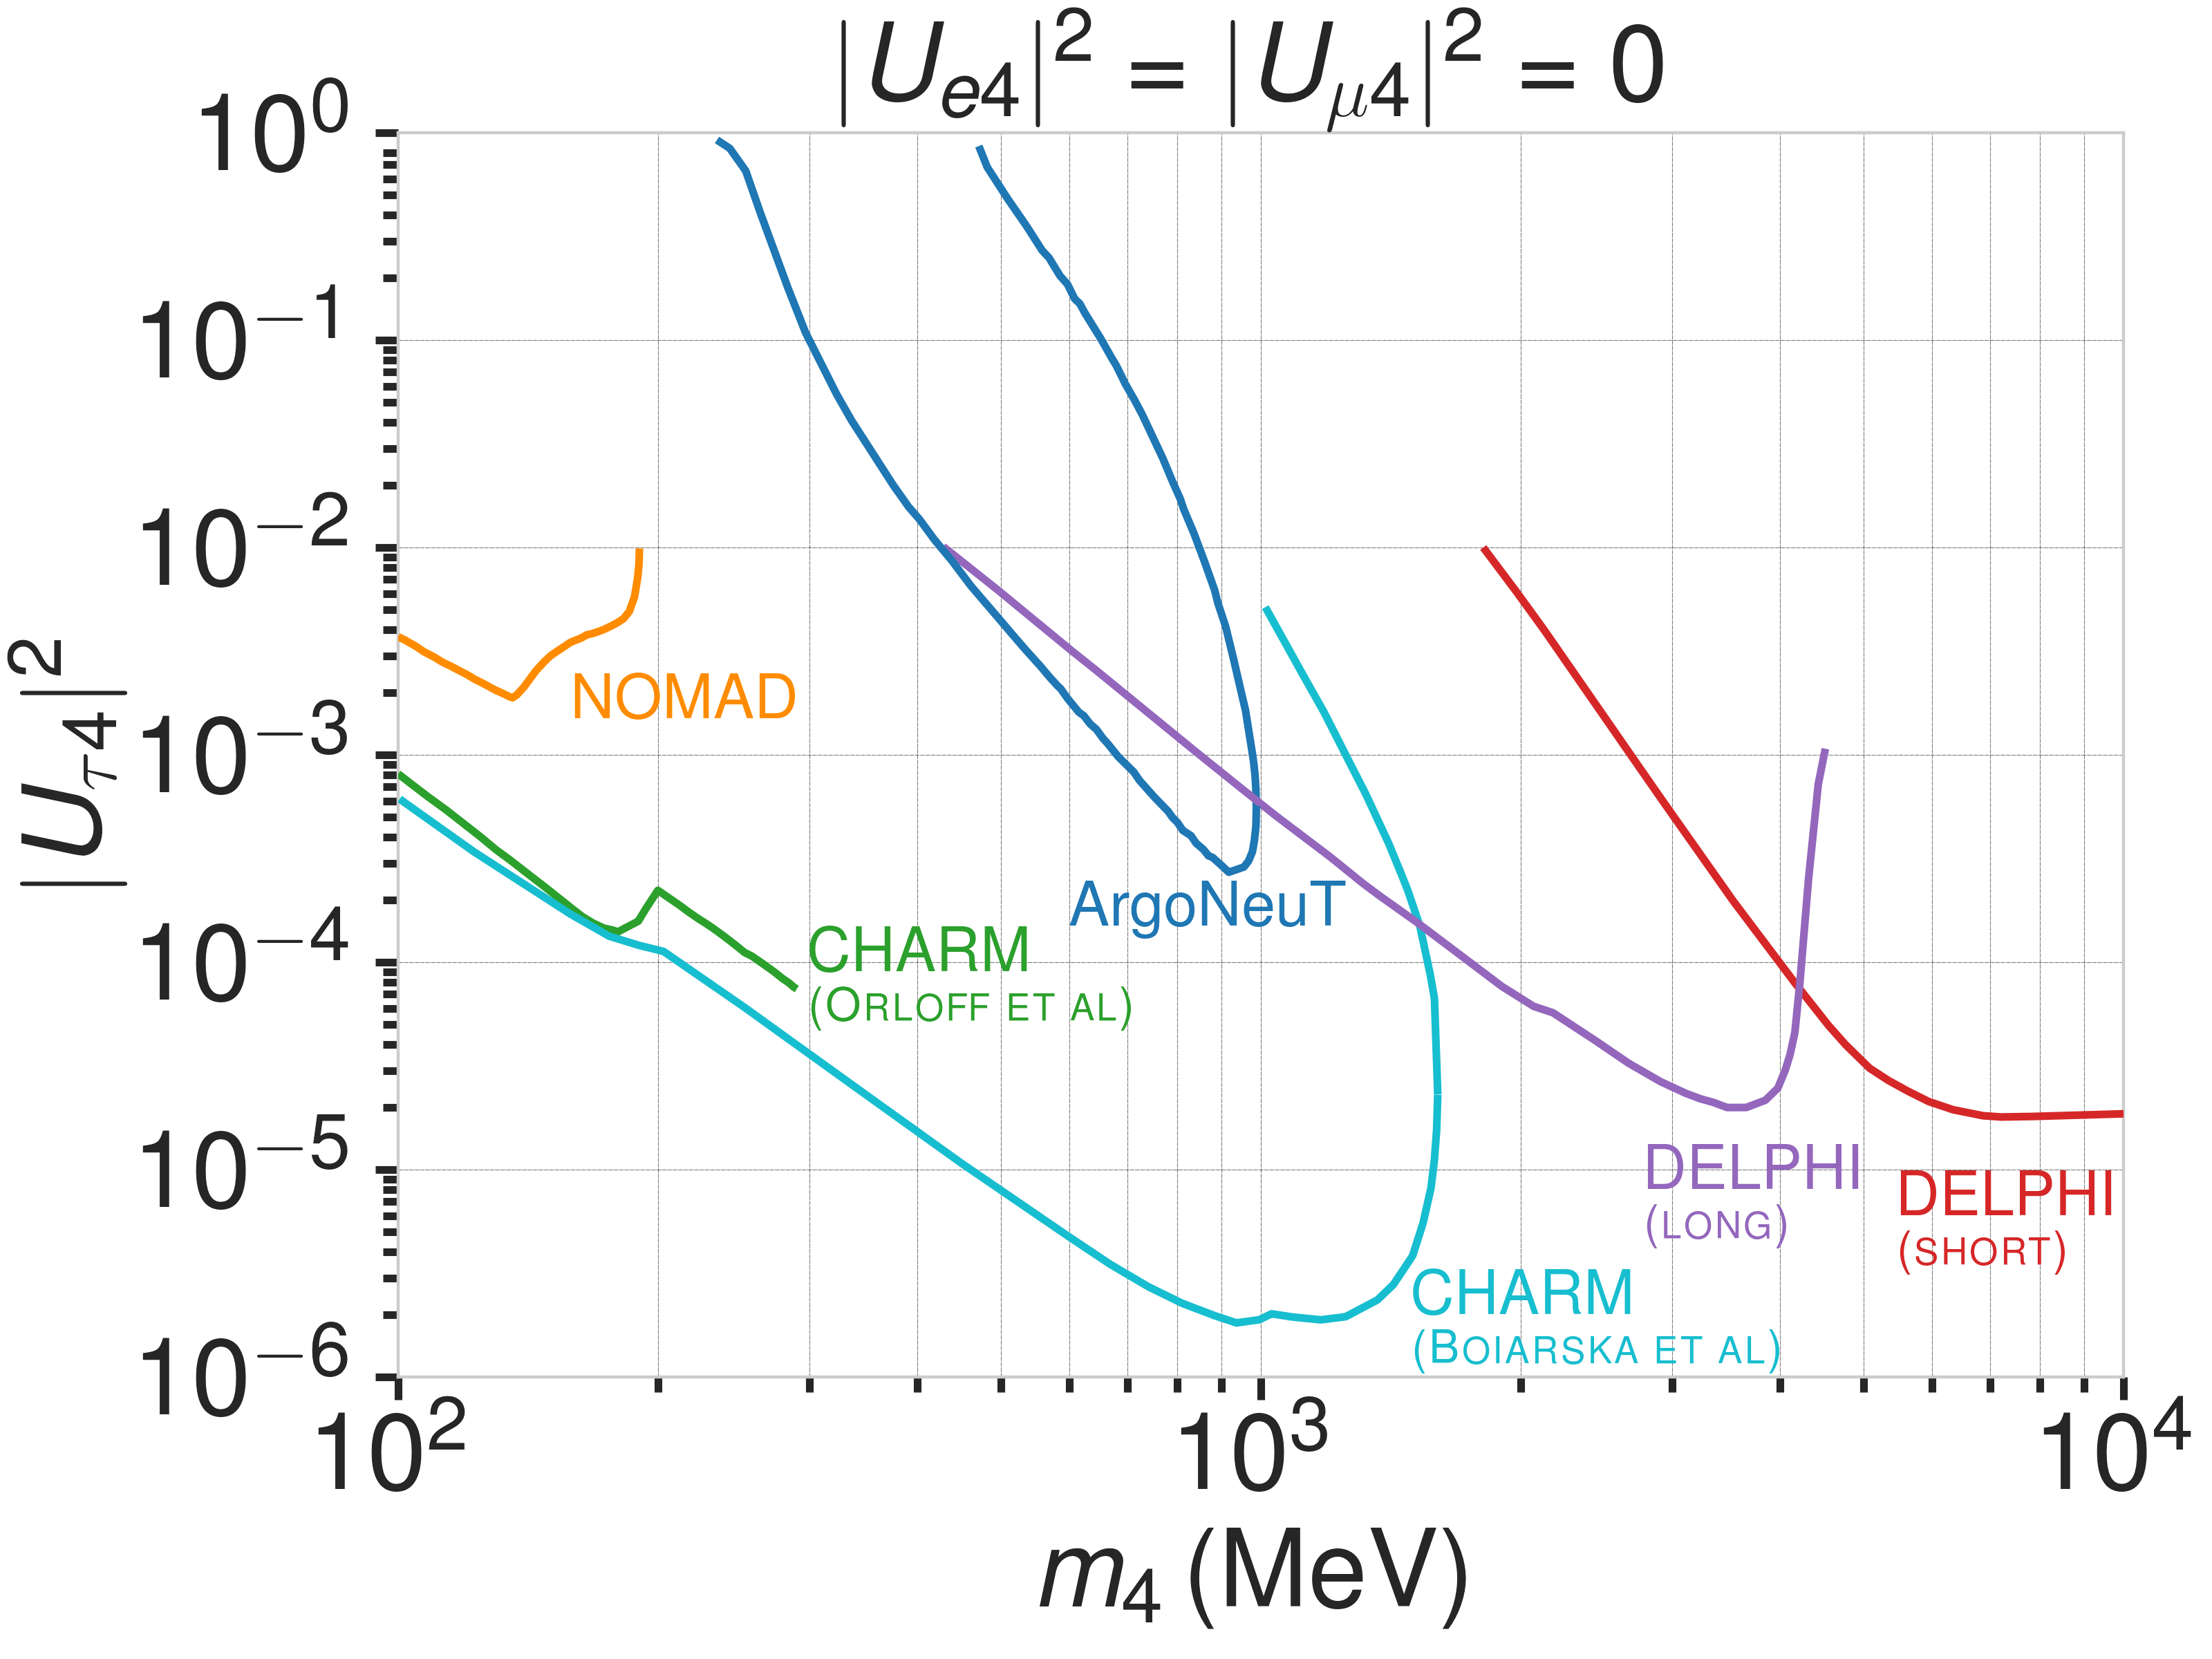
\includegraphics[width=0.49\textwidth]{figures/UtauN_custom_plots_LF_grid_white.png}
%   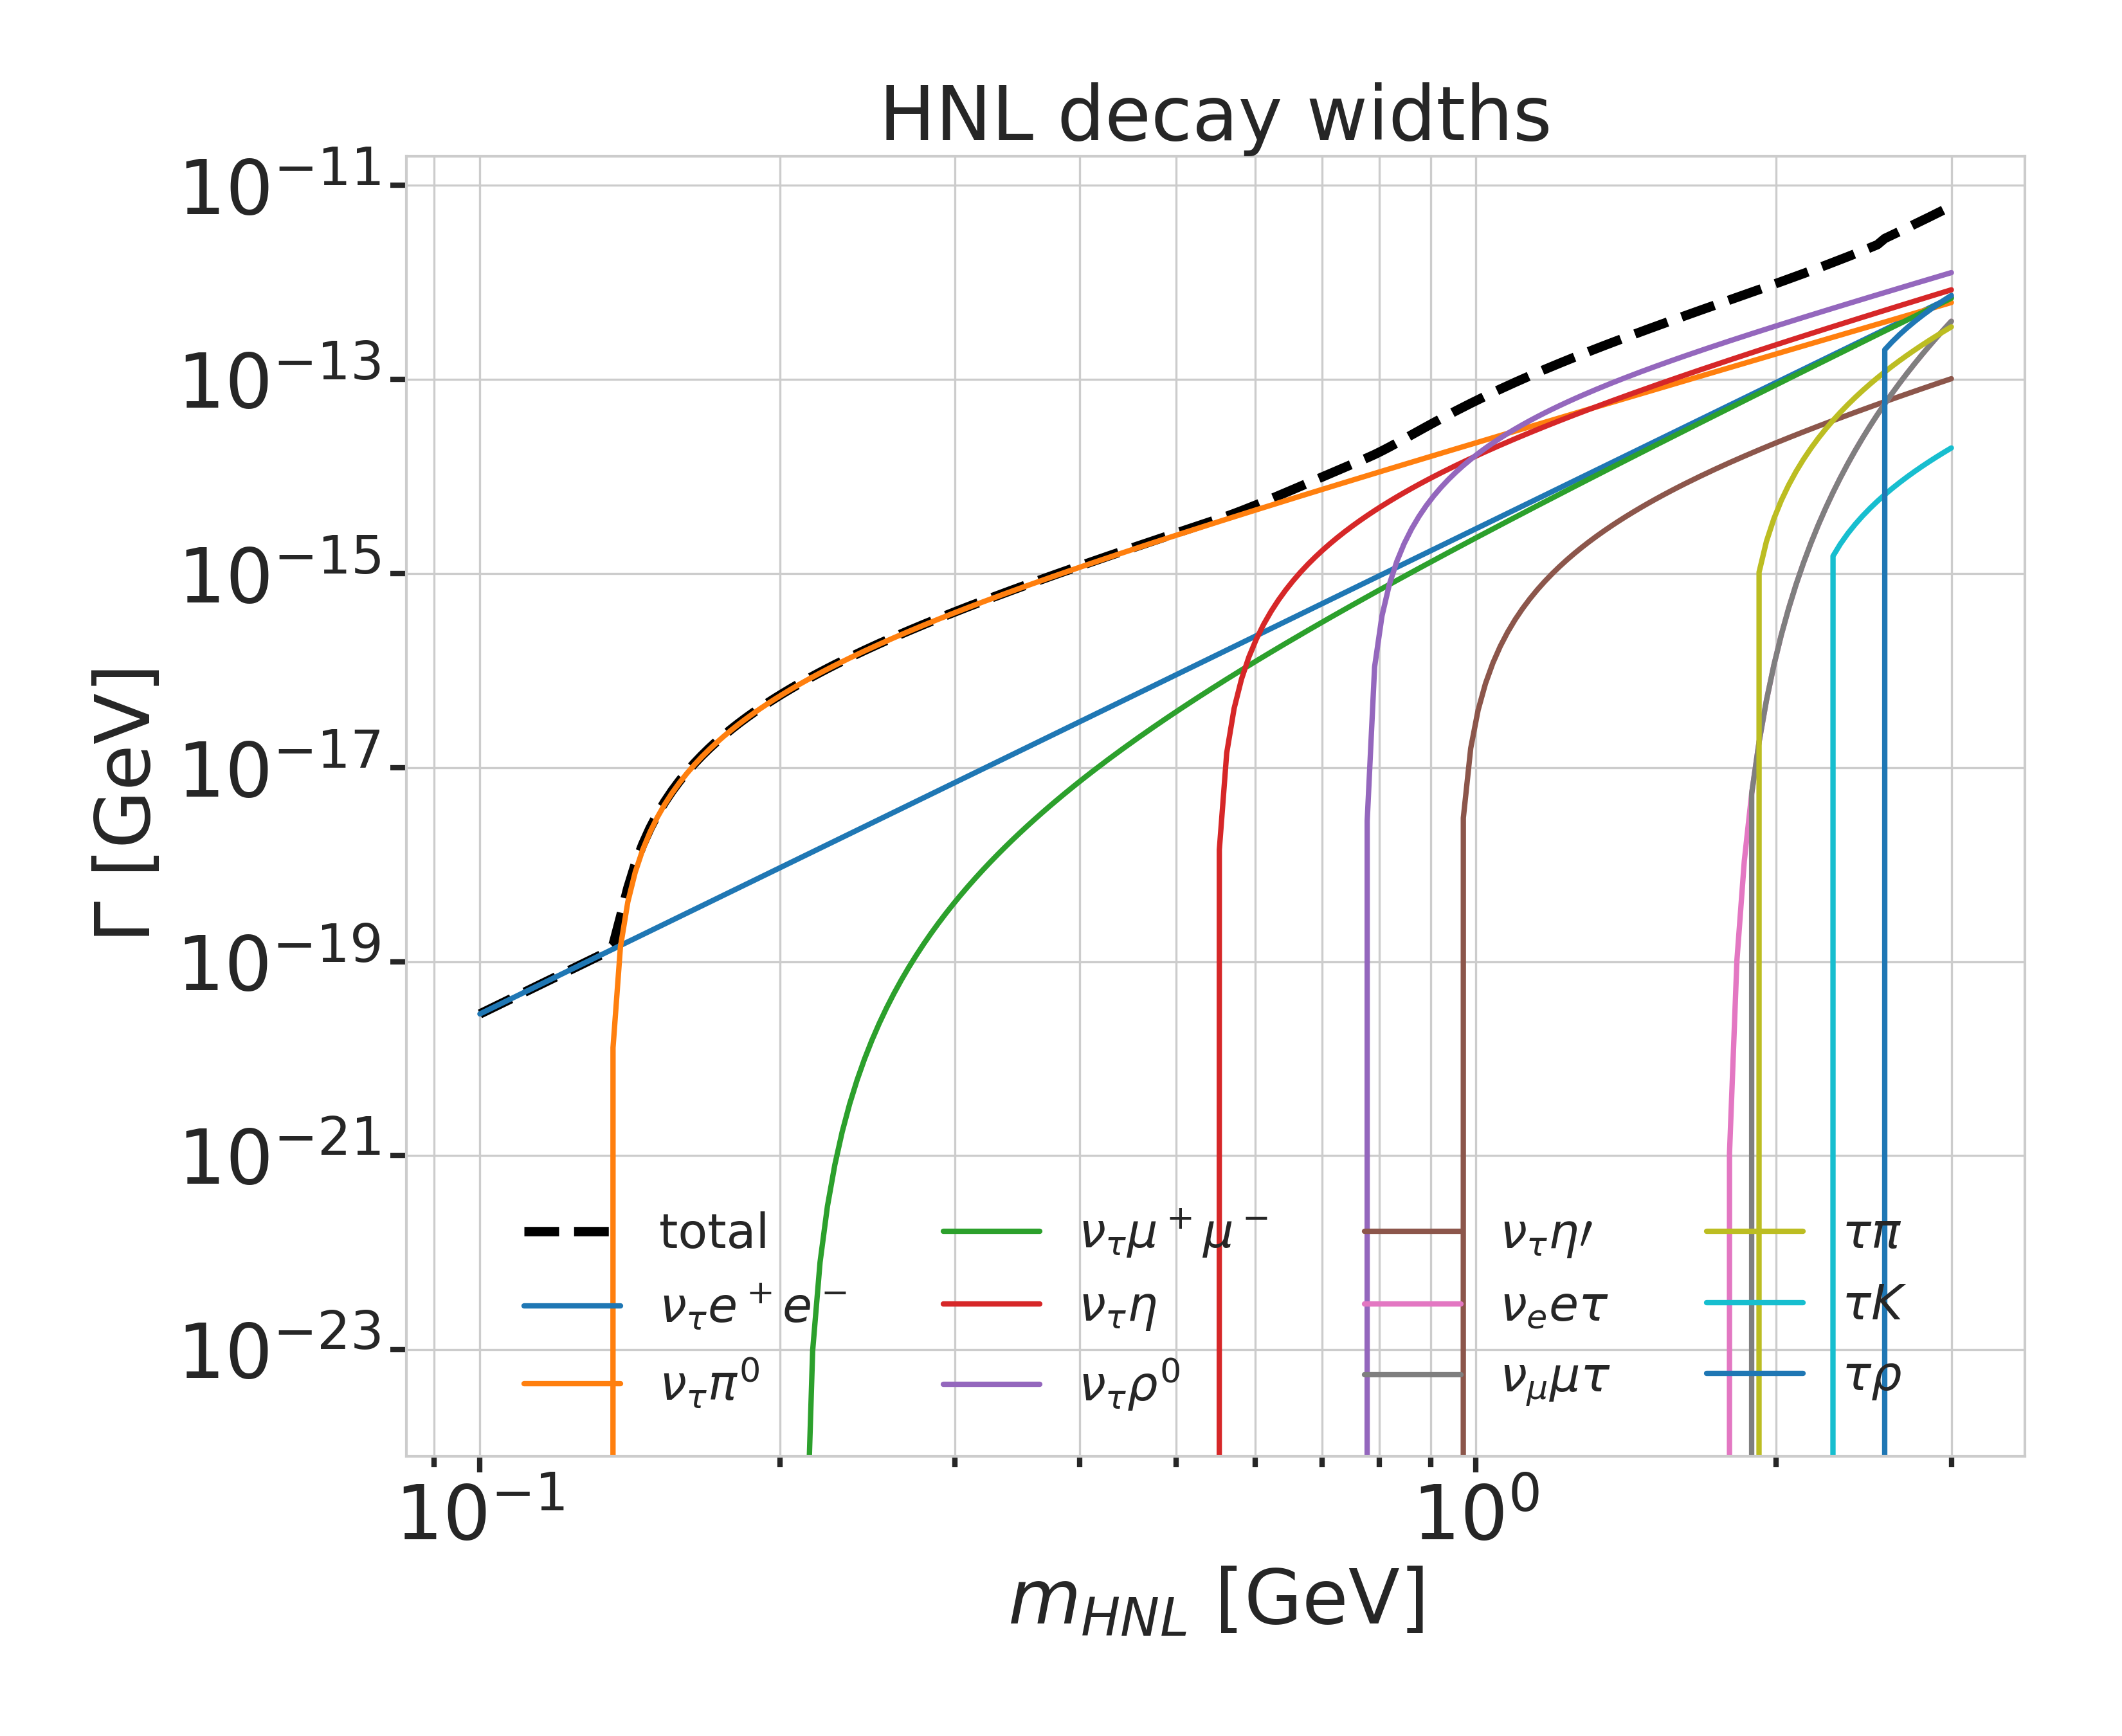
\includegraphics[width=0.49\textwidth]{figures/hnl_decay_widths_log.png}
%   \caption{Current constraints on $|U_{\tau4}^2|$ in the mass range of $[0.1,10.0]$\,GeV. Limits are from NOMAD \cite{NOMAD:2001eyx}, ArgoNeut \cite{ArgoNeuT:2021clc}, CHARM \cite{Orloff:2002de, Boiarska:2021yho}, and DELPHI \cite{DELPHI:1996qcc}.}
%   \label{fig:boundsUtau}
% \end{figure}


% \begin{figure}
%   \centering
%   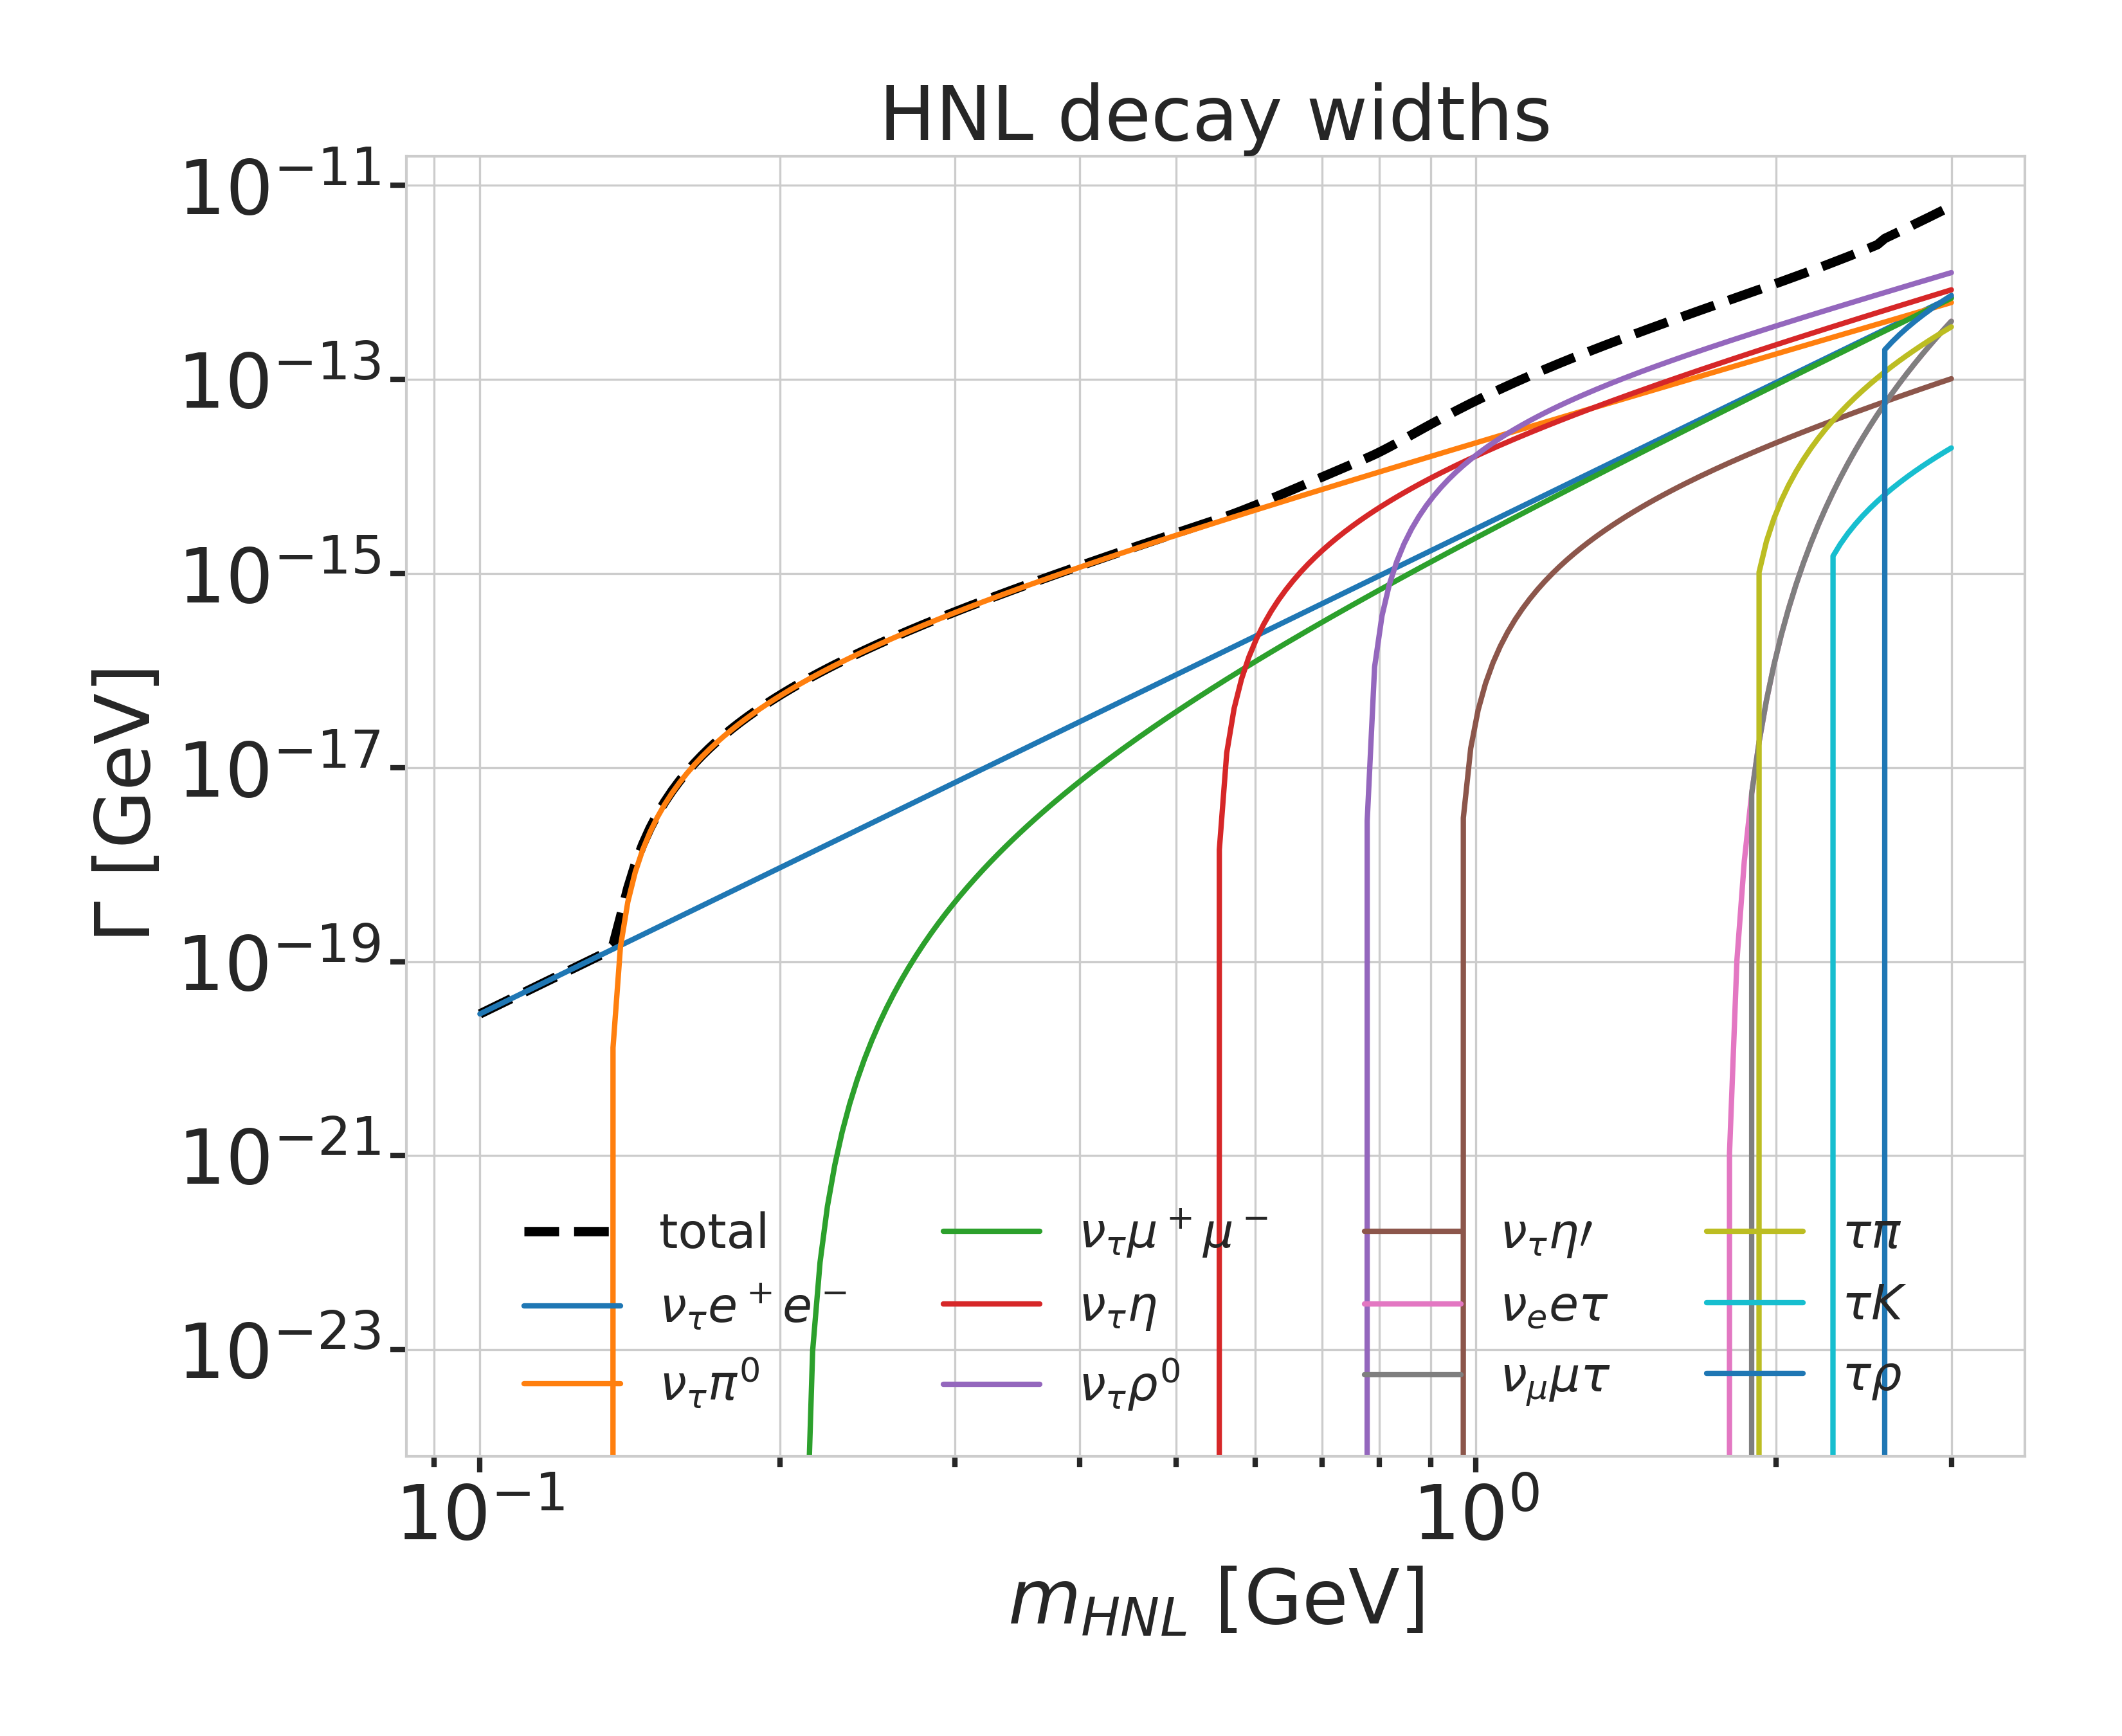
\includegraphics[width=0.7\textwidth]{figures/hnl_decay_widths_log.png}
%   \caption{Decay widths of decay modes visible in IceCube. Calculated based on the results from \cite{Gorbunov:2007ak}.}
%   \label{fig:hnl_visible_decay_widths}
% \end{figure}


\footnotesize
\bibliographystyle{JHEP}
\bibliography{MyBibFile}


\end{document}
